\documentclass[tikz,border=10pt]{standalone}
\usepackage{pgfplots}
\usetikzlibrary{patterns, backgrounds}

\begin{document}
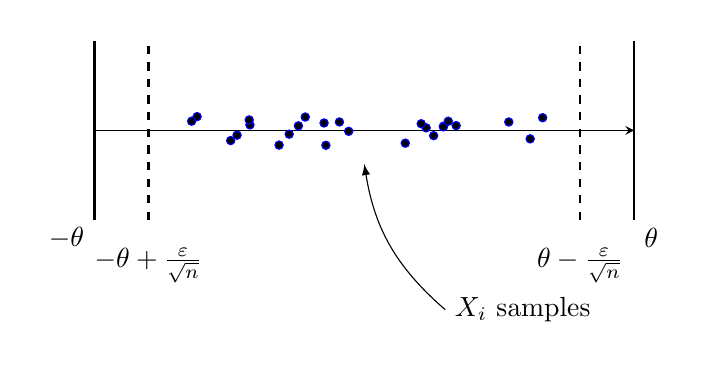
\begin{tikzpicture}[background rectangle/.style={fill=white}, show background rectangle]
  \begin{axis}[
    samples = 100,
    axis lines=middle,
    axis y line =none,
    xtick=\empty,
    ytick=\empty,
    clip=false,
    ymin=-5,
    ymax=5,
    xmin=-5,
    xmax=5, 
  ]
  % Random dots
  \addplot+[
    only marks, 
    mark=*, 
    mark options={fill=black},
    mark size=1.5pt,
    samples = 100,
    samples at={-3,-2.75,...,3},
  ] 
  (x + rand,rand/3);
  
  % Line for theta - epsilon/sqrt(n)
  \draw [dashed, thick] (axis cs:4, -2) -- (axis cs:4, 2) 
    node[pos=-0.1, below] {$\theta - \frac{\varepsilon}{\sqrt{n}}$};
  
  % Line for theta
  \draw [thick] (axis cs:5, -2) -- (axis cs:5, 2) 
    node[pos=-0.1, below, right] {$\theta$};

  \draw [thick] (axis cs:-5, -2) -- (axis cs:-5, 2) 
    node[pos=-0.1, below, left] {$-\theta$};
  
  % Line for theta + epsilon/sqrt(n)
  \draw [dashed, thick] (axis cs:-4, -2) -- (axis cs:-4, 2) 
    node[pos=-0.1, below] {$-\theta + \frac{\varepsilon}{\sqrt{n}}$};
  
  % Node for max|Xi|
  % \node[draw, circle, inner sep=2pt, fill=black] at (axis cs: 3, 4) {};
  % \node[anchor=west] at (axis cs: 3.2, 4) {max$|X_i|$};
  \draw [-latex] (axis cs: 1.5,-4) to [bend left=20] (axis cs: 0,-.75);
  \node at (axis cs: 1.5,-4) [anchor=west] {$X_i$ samples};

  \end{axis}
\end{tikzpicture}
\end{document}
